\begin{figure}[t]
\centering
\setlength{\tabcolsep}{0.8pt}
\renewcommand{\arraystretch}{0.5}
\newcommand{\lw}{0.322\linewidth}
\begin{tabular}{@{}ccc@{}}
\small display-domain loss & \small radiometric schedule & \small ground truth \\[2pt]
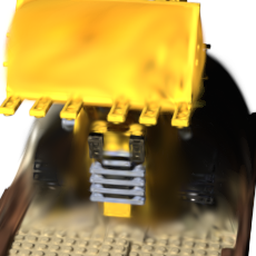
\includegraphics[width=\lw]{figures/loss_domain/lego/control_crop.png} & 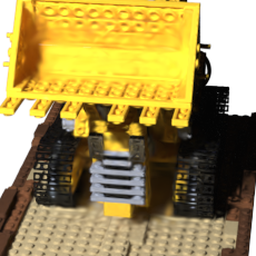
\includegraphics[width=\lw]{figures/loss_domain/lego/ours_crop.png} & 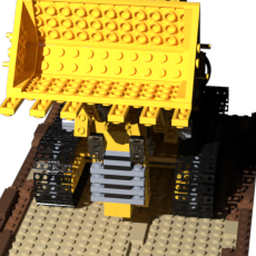
\includegraphics[width=\lw]{figures/loss_domain/lego/gt_crop.png} \\
\footnotesize 23.02\,dB & \footnotesize \textbf{30.25\,dB} & \footnotesize Lego \\[3pt]
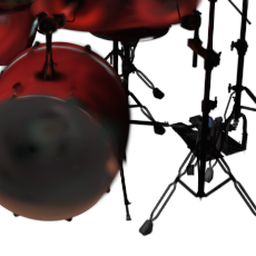
\includegraphics[width=\lw]{figures/loss_domain/drums/control_crop.png} & 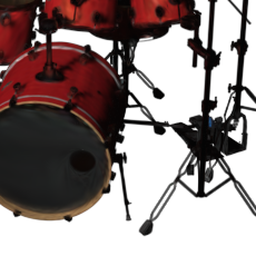
\includegraphics[width=\lw]{figures/loss_domain/drums/ours_crop.png} & 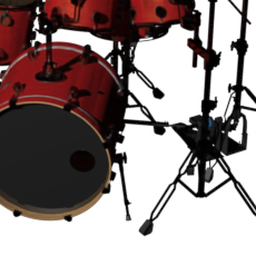
\includegraphics[width=\lw]{figures/loss_domain/drums/gt_crop.png} \\
\footnotesize 24.10\,dB & \footnotesize \textbf{30.10\,dB} & \footnotesize Drums \\[3pt]
\end{tabular}
\caption{\textbf{Loss domain and geometry.} Two runs that share initialization, schedule, random state and every other setting, differing only in whether the loss is computed on display-encoded or (after the annealed warm-up) linear radiance; 16k iterations, PSNR over 200 held-out training views. All 200 views improve on both scenes.}
\label{fig:loss_domain}
\end{figure}
